\documentclass[dvipdfmx]{beamer}

\usepackage{graphicx,color}

%読めない、意味分からないのでコメントアウト。なくても動くし
%\usepackage{siunitx}

\usepackage{comment}
\usepackage{listings, jlisting}
\usepackage{fancyvrb}
\usepackage{subfigure}
\usepackage[font=footnotesize]{caption}

% 図表番号を振る
\setbeamertemplate{caption}[numbered]

% 下の図表番号のスペースを除去
\setlength\abovecaptionskip{0.5em}

\newenvironment{wideitemize}{\itemize\setlength{\itemsep}{1em}}{\enditemize}
\newenvironment{wideitemize2}{\itemize\setlength{\itemsep}{0.2em}}{\enditemize}
\newenvironment{widedescription}{\description\setlength{\itemsep}{1em}}{\enddescription}
\newenvironment{widedescription2}{\description\setlength{\itemsep}{0.2em}}{\enddescription}

\lstset{language=C++,
    basicstyle=\ttfamily\scriptsize,
    keywordstyle=\color{blue}\ttfamily,
    stringstyle=\color[cmyk]{0,0.6,1,0.2}\ttfamily,
    commentstyle=\color[cmyk]{1,0.4,1,0}\ttfamily,
    identifierstyle=\color[cmyk]{0,1,0.1,0.8}\ttfamily,
    morecomment=[l][\color{magenta}]{\#},
    breaklines = true
}

%\usetheme{Rochester}
\usetheme{Madrid}
\usecolortheme{seahorse}

\title[2015年度初年次ゼミ問題]{具体的な問題}
\subtitle{}
\author[遠藤 亘 岩崎 慎太郎]{遠藤 亘 岩崎 慎太郎}
\institute[田浦研]{情報理工学系研究科 修士1年 田浦研究室}
\date{2015-05-07}

\begin{document}

\begin{frame}
\titlepage
\end{frame}


%%%%%%%%%%%%%%%%%%%%%%%%%%%%%%%%%%%%%%%%%%%%%%%%%%%%%%%%%%%%%%%%%%%%%%%%%%%%%%%%%%%%%%%%%%%%%%%%%%%%%%%%%%%%

\begin{frame}{問題1}{探査衛星とスイングバイ}
\begin{columns}[t]
\begin{column}{0.7\textwidth}
\begin{wideitemize}
	\item 太陽系外に探査機を打ち出したい。打ち上げ日時と位置を求めよ。
	\begin{wideitemize2}
		\item (ボイジャーの打ち上げられた)1970年代に打ち上げる。
		\item 最初のスイングバイまでに太陽を一周しない。
		\item 地上発射時の初速は14.2km/sで、地球を黄道面で切った時の断面円周上のどこから打ち上げても良い
		\item 探査機の重さは750kg。ロケットからの分離は考えない
		\item 惑星(太陽~土星まで)は太陽を中心に円軌道を描き、全て同一平面上で運動するとする
		\item 地球の自転の影響を無視して地上から垂直に打ち上げたとする
	\end{wideitemize2}
\end{wideitemize}

\end{column}
\begin{column}{0.3\textwidth}
\begin{figure}[htbp]
    \centering
    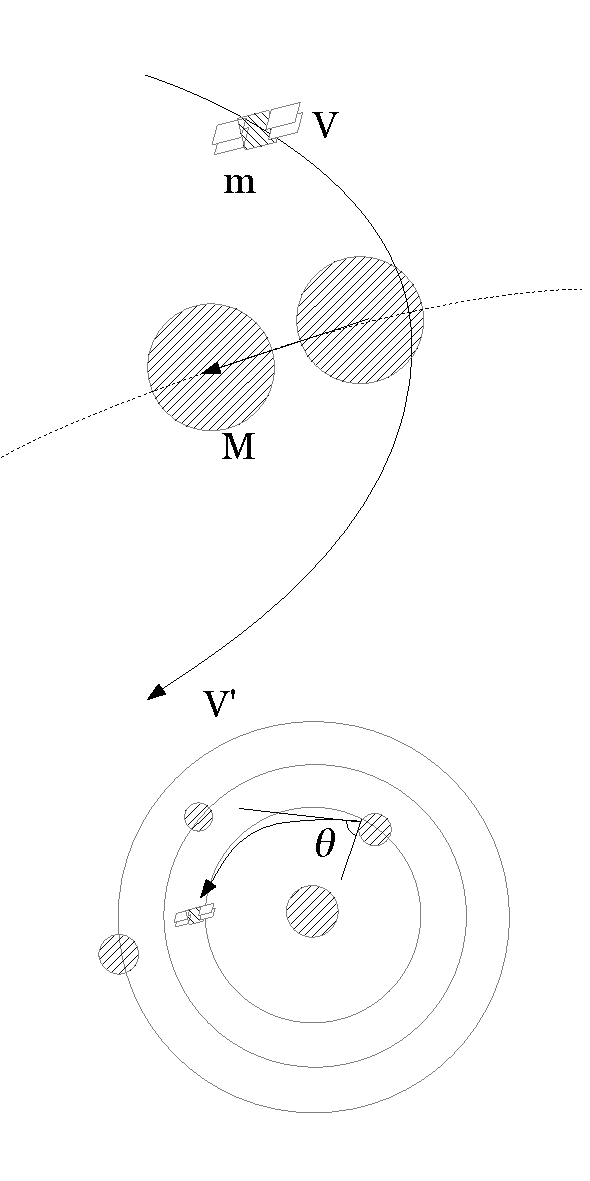
\includegraphics[bb=0mm 0mm 100.0mm 170.0mm, scale=0.35, type=pdf]{img/problem1.pdf}
\end{figure}
\end{column}
\end{columns}
\end{frame}

%%%%%%%%%%%%%%%%%%%%%%%%%%%%%%%%%%%%%%%%%%%%%%%%%%%%%%%%%%%%%%%%%%%%%%%%%%%%%%%%%%%%%%%%%%%%%%%%%%%%%%%%%%%%

\begin{frame}{問題2}{飛行距離}
\begin{columns}[t]
\begin{column}{0.7\textwidth}
\begin{wideitemize}
	\item ペットボトルロケットを遠くまで飛ばしたい。最適な水の量、圧力、打ち上げ角度はいくつか?
	\begin{wideitemize2}
		\item 標準大気圧、25度で乾燥しており、無風
		\item 空気は粘性のない、比熱比1.4の理想気体
		\item ペットボトルは半径45mmで容積1.5Lの円柱で、耐圧0.6MPa
		\item ノズルは直径4mm、ロケットの先端は頂角60度の円錐
		\item 水を除いたロケット全体の重さは150g
		\item 翼はなく、揚力は考えない
	\end{wideitemize2}
\end{wideitemize}

\end{column}
\begin{column}{0.3\textwidth}
\begin{figure}[htbp]
    \centering
    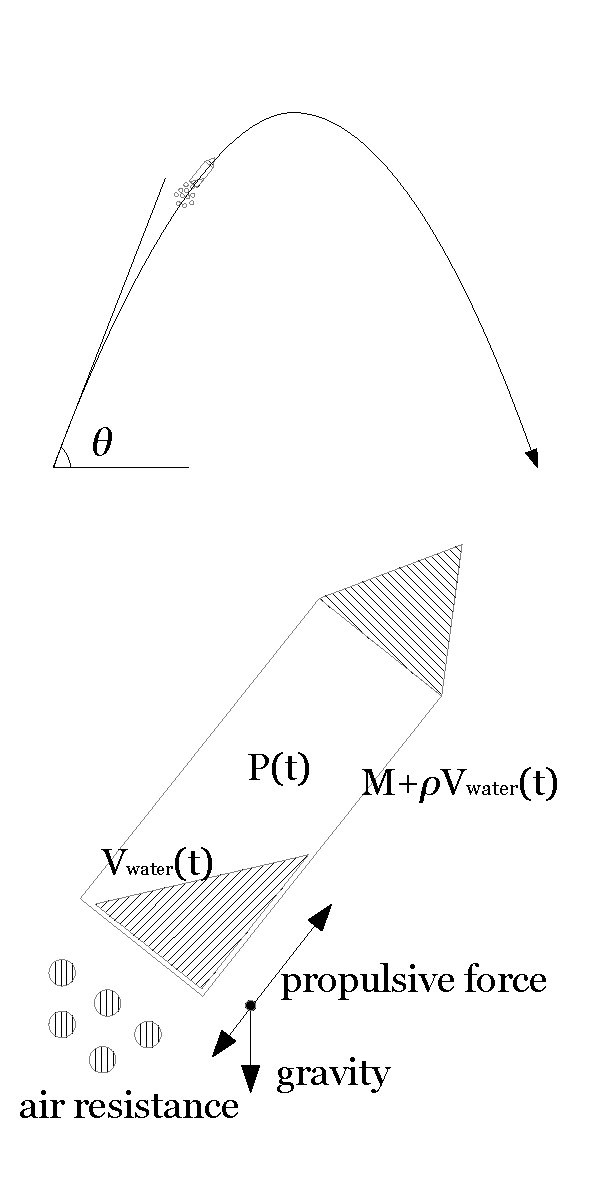
\includegraphics[bb=0mm 0mm 100.0mm 170.0mm, scale=0.35, type=pdf]{img/problem2.pdf}
	% http://atsites.jp/yoshitoharada/1150_Water-rocket1.jpg
\end{figure}
\end{column}
\end{columns}
\end{frame}

%%%%%%%%%%%%%%%%%%%%%%%%%%%%%%%%%%%%%%%%%%%%%%%%%%%%%%%%%%%%%%%%%%%%%%%%%%%%%%%%%%%%%%%%%%%%%%%%%%%%%%%%%%%%

\begin{frame}{問題3}{結晶構造}
\begin{columns}[t]
\begin{column}{0.7\textwidth}
\begin{wideitemize}
	\item スピネル$Mg Al_2 O_4$の結晶構造を、とても簡便な分子動力学的な計算によって求めたい。
	スピネルの密度はどれくらいの精度で計算できるだろうか?
	\begin{wideitemize2}
		\item イオン半径等のパラメータは適当なものを用いてよい。
		\item 圧力などは、適当なものを用いること。
	\end{wideitemize2}

\end{wideitemize}

\end{column}
\begin{column}{0.3\textwidth}
\begin{figure}[htbp]
    \centering
    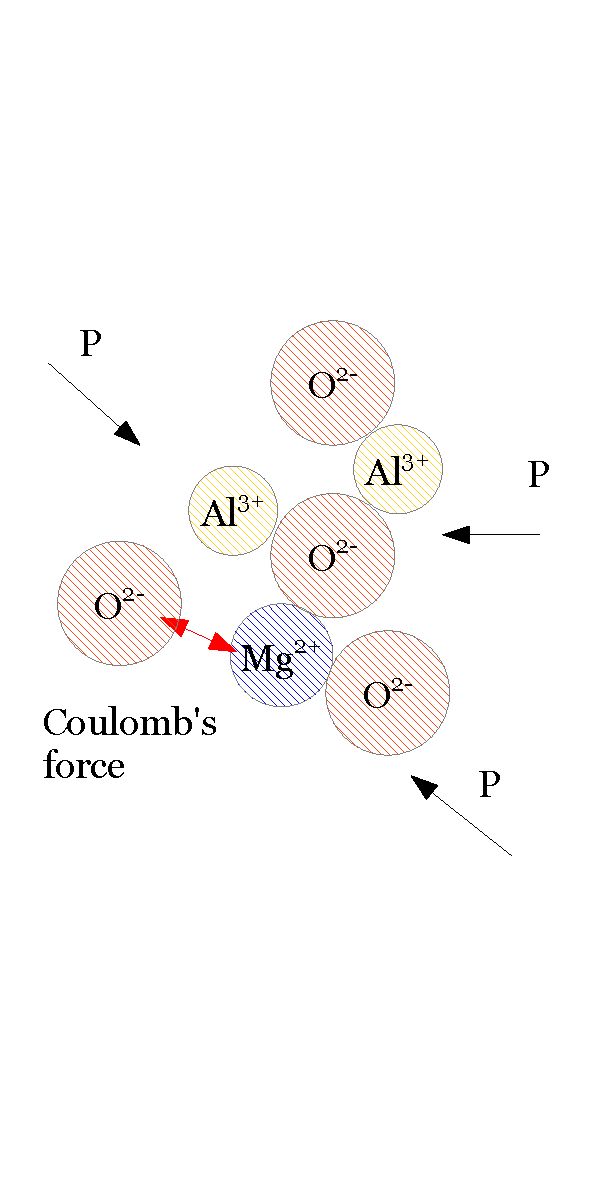
\includegraphics[bb=0mm 0mm 100.0mm 170.0mm, scale=0.35, type=pdf]{img/problem3.pdf}
\end{figure}
\end{column}
\end{columns}
\end{frame}

%%%%%%%%%%%%%%%%%%%%%%%%%%%%%%%%%%%%%%%%%%%%%%%%%%%%%%%%%%%%%%%%%%%%%%%%%%%%%%%%%%%%%%%%%%%%%%%%%%%%%%%%%%%%

\begin{frame}{問題4}{歯車}
\begin{columns}[t]
\begin{column}{0.7\textwidth}
\begin{wideitemize}
	\item 歯数5同士でかみ合う二次元の歯車を設計し、片方を一定角速度で回転させたときのもう片方の角速度の滑らかさを、シミュレーションで評価せよ。
	\begin{wideitemize2}
		\item 軸間距離などを変えた際に、歯車の形によってどのような変化が生じるだろうか。
		\item 図のようにカクカクした歯車を作ると、角速度はどのような変化をするだろうか。
	\end{wideitemize2}

\end{wideitemize}

\end{column}
\begin{column}{0.3\textwidth}
\begin{figure}[htbp]
    \centering
    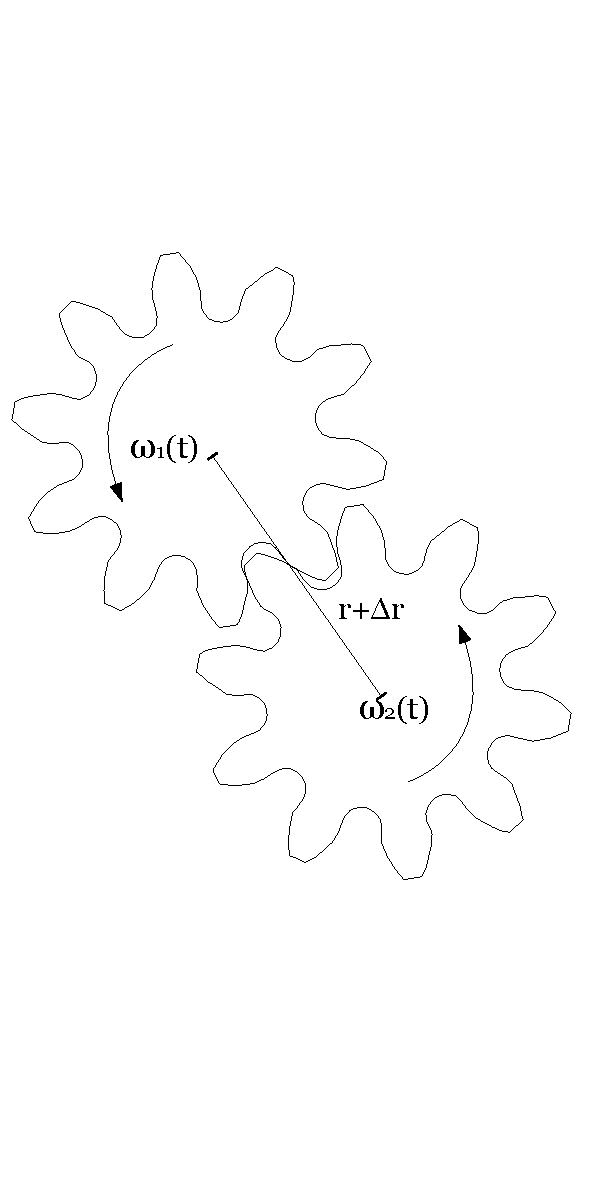
\includegraphics[bb=0mm 0mm 100.0mm 170.0mm, scale=0.35, type=pdf]{img/problem4.pdf}
\end{figure}
\end{column}
\end{columns}
\end{frame}

%%%%%%%%%%%%%%%%%%%%%%%%%%%%%%%%%%%%%%%%%%%%%%%%%%%%%%%%%%%%%%%%%%%%%%%%%%%%%%%%%%%%%%%%%%%%%%%%%%%%%%%%%%%%

\begin{frame}{問題5}{空間消音}
\begin{columns}[t]
\begin{column}{0.7\textwidth}
\begin{wideitemize}
	\item 救急車のサイレン音打消しをモデルとして、空間の消音をしたい。消音スピーカーから各々どのような波を出せばよいか
	\begin{wideitemize2}
		\item 幅(x軸)$1.6m$、長さ(y軸)$3.6m$、高さ(z軸)$2m$の大きさの直方体を考え、上面端に$(0, 0, 0)$座標を置く
		\item 960Hzで振幅1の正弦波を出すサイレンが$(0.8,1.8,0)$の位置にある
		\item 消音スピーカーは、高さ$1.6m$、壁面から$0.2m$離れた位置に4つ置く
		\item $(0.6, 2.0, 2.0)$、$(1.0, 2.0, 2.0)$、$(1.0, 2.4, 2.0)$、$(0.6, 2.4, 2.0)$を底面とし、高さが$0.4m$の立方体の空間でエネルギーを最小化する
		\item 標準大気圧で、乾燥しており、温度は20度とする。
	\end{wideitemize2}

\end{wideitemize}

\end{column}
\begin{column}{0.3\textwidth}
\begin{figure}[htbp]
    \centering
    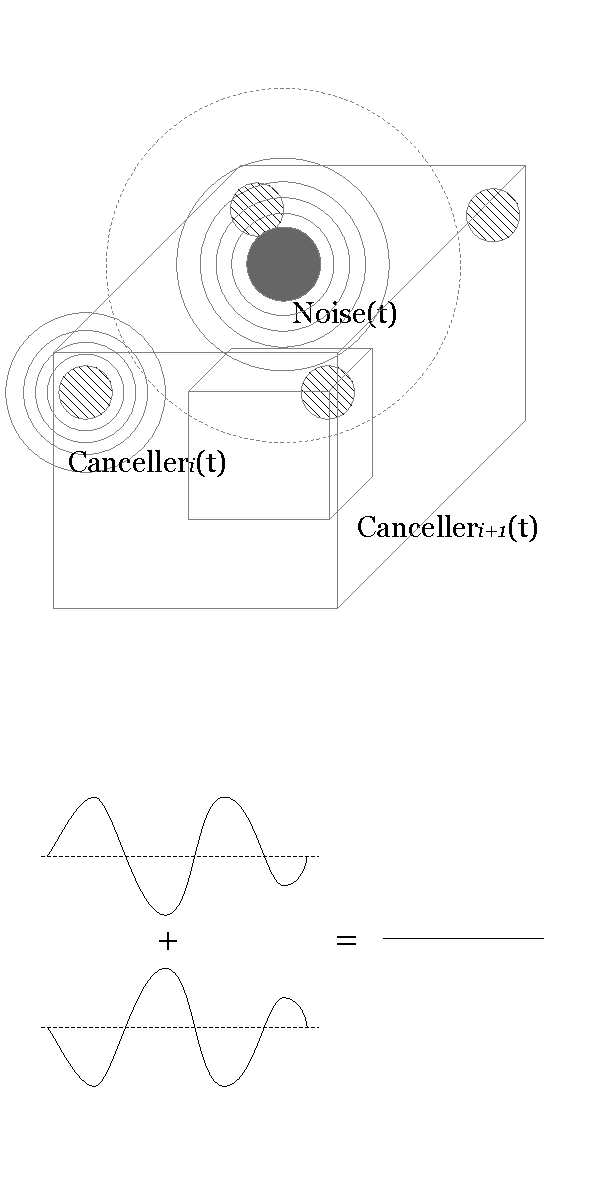
\includegraphics[bb=0mm 0mm 100.0mm 170.0mm, scale=0.35, type=pdf]{img/problem5.pdf}
\end{figure}
\end{column}
\end{columns}
\end{frame}

%%%%%%%%%%%%%%%%%%%%%%%%%%%%%%%%%%%%%%%%%%%%%%%%%%%%%%%%%%%%%%%%%%%%%%%%%%%%%%%%%%%%%%%%%%%%%%%%%%%%%%%%%%%%

\begin{frame}{問題6}{翼へ...}
\begin{columns}[t]
\begin{column}{0.7\textwidth}
\begin{wideitemize}
	\item 二次元翼として、ジューコフスキー翼の迎え角と揚力の関係を求めたい。
	\item だが、少し難しすぎるので、平面板間を流れる二次元的な流体に図のように正方形の障害物を置いた際の流れの乱れを
	シミュレーションせよ。
	\begin{wideitemize2}
		\item 非圧縮性流体を仮定する。適当な流体(空気、あるいは水)を仮定せよ。
		\item 管の太さ、あるいは障害物の大きさを変えるとどのようなふるまいをするだろうか。
	\end{wideitemize2}
\end{wideitemize}

\end{column}
\begin{column}{0.3\textwidth}
\begin{figure}[htbp]
    \centering
    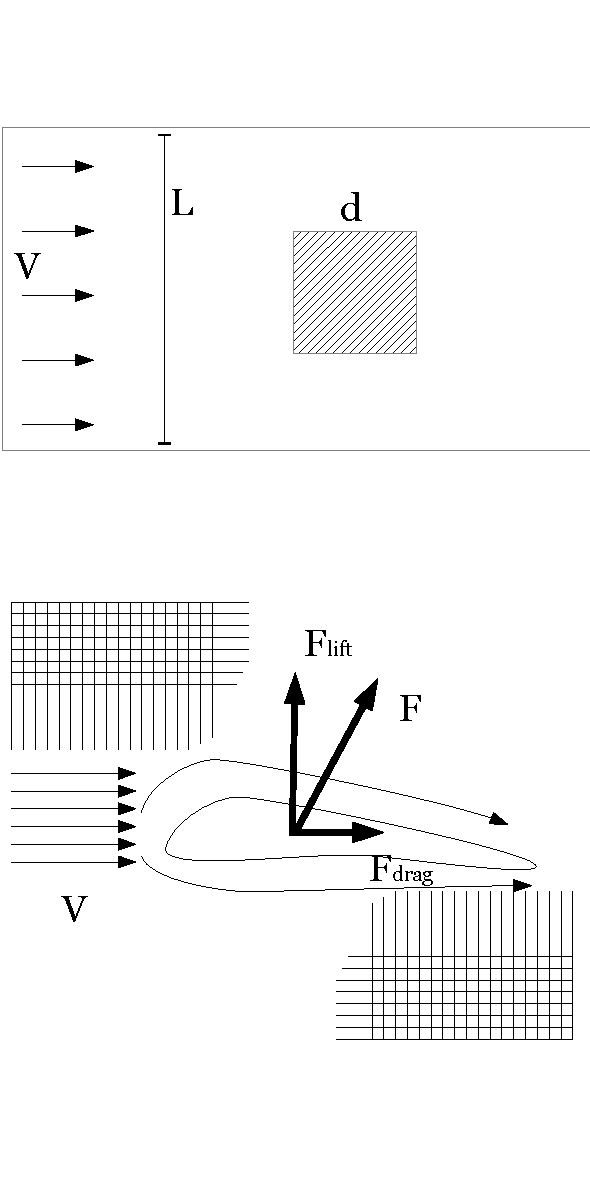
\includegraphics[bb=0mm 0mm 100.0mm 170.0mm, scale=0.35, type=pdf]{img/problem6.pdf}
\end{figure}
\end{column}
\end{columns}
\end{frame}

%%%%%%%%%%%%%%%%%%%%%%%%%%%%%%%%%%%%%%%%%%%%%%%%%%%%%%%%%%%%%%%%%%%%%%%%%%%%%%%%%%%%%%%%%%%%%%%%%%%%%%%%%%%%

\begin{frame}{問題7}{ベンゼン}
\begin{columns}[t]
\begin{column}{0.7\textwidth}
\begin{wideitemize}
	\item ベンゼン分子の電子軌道を計算することで、ベンゼンの炭素-炭素間結合が「1.5重結合」であることを確認したい。
	\begin{wideitemize2}
		\item ハートリー・フォック法を用いること。
		\item 基底関数系に適当なガウス基底を用いること。
		\item ベンゼン分子中の各原子の位置は予め与えてよい。
	\end{wideitemize2}
\end{wideitemize}

\end{column}
\begin{column}{0.3\textwidth}
\begin{figure}[htbp]
    \centering
    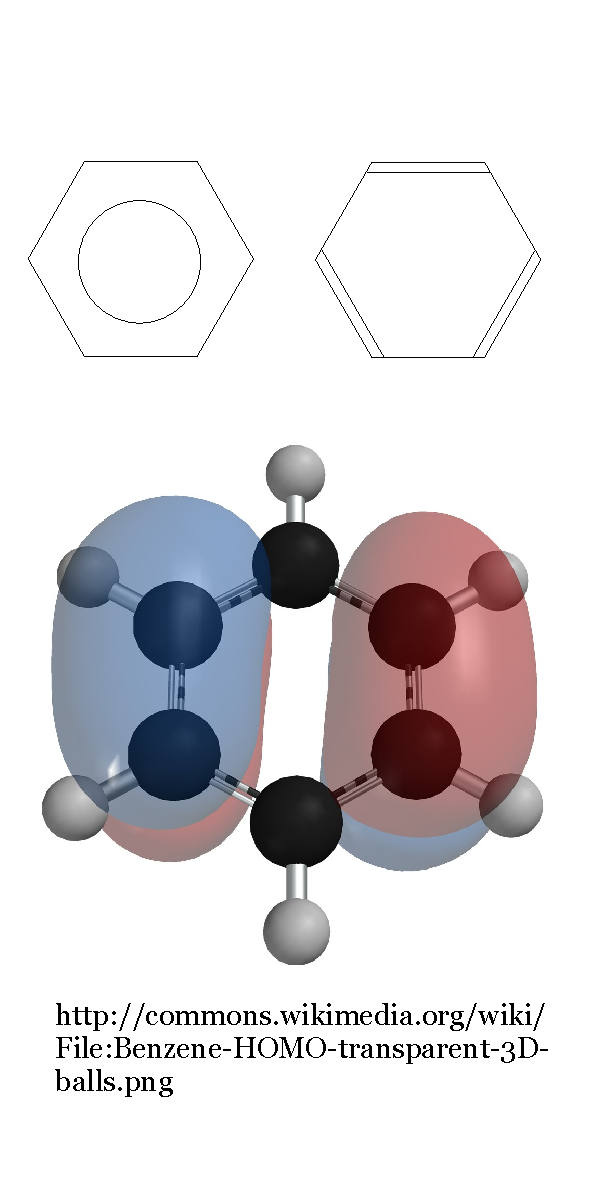
\includegraphics[bb=0mm 0mm 100.0mm 170.0mm, scale=0.35, type=pdf]{img/problem7.pdf}
\end{figure}
\end{column}
\end{columns}
\end{frame}


%%%%%%%%%%%%%%%%%%%%%%%%%%%%%%%%%%%%%%%%%%%%%%%%%%%%%%%%%%%%%%%%%%%%%%%%%%%%%%%%%%%%%%%%%%%%%%%%%%%%%%%%%%%%

\begin{frame}{問題:まとめ}
\begin{wideitemize}
\item 探査衛星とスイングバイ
\item ペットボトルロケットの飛行距離
\item スピネルの結晶構造
\item 歯車の回転
\item 空間消音
\item 流体の流れ
\item ベンゼンの電子軌道
\end{wideitemize}
\end{frame}



\end{document}

